\usepackage{slashbox,pict2e}
\newpage
\section{Проектирование}
\label{sec:designing}
В разделе 2.1. представлены функциональные и нефункциональные требования к системе. В разделе 2.2. описаны варианты использования системы. В разделе в разделе 2.3. представлена архитектура приложения, а в разделе 2.4. показан графический интерфейс, а в разделе 2.5. сравниваются различные алгоритмы выявления фиктивных аккаунтов.

\vspace{1.5em}
\subsection{Требования к системе}
\label{subsec:fotmalDefinition}
\textbf{Функциональные требования}

Функциональные требования определяют функциональность программного обеспечения, то есть описывают, какое поведение должна предоставлять разрабатываемое приложение

\textbf{Нефункциональные требования}

К нефункциональным требованиям системы относятся свойства, которыми она должна обладать. Например, удобство использования, безопасность, расширяемость и т.д.

\vspace{1.5em}
\subsection{Варианты использования системы}
\label{subsec:Variants}
Описание способов взаимодействия с системой, кто с ней может работать, каким образом.

\vspace{1.5em}
\subsection{Архитектура приложения}
\label{subsec:Architecture}
Показать модули приложения, расписать то, что делает каждый из них.

\vspace{1.5em}
\subsection{Графический интерфейс}
\label{subsec:Graphic}
Представление графического интерфейса программной системы.

\vspace{1.5em}
\subsection{Сравнение алгоритмов}
\label{subsec:Algoritm}
Для нахождения наилучшего алгоритма выявления фиктивных аккаунтов были разработаны пробные модели, а после найдены их критерии качества. 

Первое, что было сделано - это извлечение признаков, по которым проводилась кластеризация. Признаки:
\begin{itemize}
    \item user\_id: уникальный идентификатор пользователя. Используется для идентификации каждого аккаунта;
    \item username\_length: длина имени пользователя;
    \item numbers\_in\_name: переменная, которая означает наличие цифр в имени пользователя. Если нет – ставится 0, иначе – 1;
    \item email\_length: длина email;
    \item matching\_names: переменная, которая означает совпадение username с email по определенному порогу сходства (в случае несовпадения 0, иначе – 1);
    \item pattern\_email: продходит ли email по шаблону user@domain.com (в случае прохождения по парамтру 0, иначе – 1);
    \item country: проверка, указана ли страна (если не указана - 0, иначе - 1);
    \item date\_last\_email: проверка даты последнего отправленного email. Если она есть – 1, иначе – 0;
    \item date\_registered: дата регистрации аккаунта;
    \item date\_last\_login: дата последнего входа в аккаунт;
    \item matching\_dates: характеристика, совпадают ли даты послегнего входа в аккаунт и даты регистрации.
\end{itemize}

Далее подробнее рассмотрим алгоритмы кластеризации, которые были использованы для нахождения аномалий в виде фиктивных аккаунтов. 

\vspace{1.5em}
\textbf{Алгоритм изолированного леса}

Была произведена подготовка данных в виде заполнения пропущенных значений средним значением по столбцу. Была реализована нормализация признаков: они преобразованы в данные в диапазоне от 0 до 1. Установлена ожидаемая доля аномалий - 5\%.
Аномалии (данные с индексом -1) были занесены в файл, а также создано графическое изображение для результатов кластеризации (рис. ~\ref{ris:isolation-forest}).

\begin{figure}[!ht]
    \center{\includegraphics[width=1\linewidth]{image}}
    \includegraphics[scale=0.5]{Курсовая работа/pic/anomaly_isolation-forest0.png}
    \caption{Кластеризация методом изолированного леса}
    \label{ris:isolation-forest}
\end{figure}

После этого были произведены расчеты метрик алгоритма, с использованием ячеек матрицы ошибок (табл. ~\ref{tabular:tableIsolationForest}), где TP – число объектов, предсказанных моделью как положительные, которые действительно являются положительными, TN – число объектов, предсказанных моделью как отрицательные, которые действительно являются отрицательными, FP – число объектов, предсказанных моделью как положительные, которые на самом деле являются отрицательными, FN – число объектов, предсказанных моделью как отрицательные, которые на самом деле являются положительными. 

\begin{table}[!ht]
    \onehalfspacing \caption{Прогноз алгоритма}
    \medskip
        \begin{tabular}{|c|c|}
        \hline
            True Positive & 7\\  \hline 
            True Negative & 151\\  \hline 
            False Positive & 6\\  \hline 
            False Negative & 90\\  \hline 
        \end{tabular}
    \label{tabular:tableIsolationForest}
\end{table}

Для оценки качества работы алгоритма необходимо ввести метрики accuracy (аккуратность), precision (точность) и recall (полнота). Первая показывает долю верно классифицированных объектов, вторая – долю объектов, которые модель классифицировала как положительные, и которые действительно являются положительными, а третья – долю объектов положительного класса, которые модель определила правильно. Рассчитаем их значения.

$$
accuracy = \frac{TP+TN}{TP+TN+FP+FN} = 0,63
$$

$$
precision = \frac{TP}{TP+FP} =  0,62
$$

$$
recall = \frac{TP+TN}{TP+FN} = 0,08
$$

$$
F = 2\cdot \frac{precision \cdot recall}{precision+recall} = 0,14
$$

\vspace{1.5em}
\textbf{Алгоритм иерархической кластеризации}

Была произведена подготовка данных в виде заполнения пропущенных значений средним значением по столбцу. Была реализована нормализация признаков: они преобразованы в данные в диапазоне от 0 до 1. Была произведена сортировка по username\_length. Создана матрица расстояний с методом Single Linkage, так как он сильнее реаширует на выбросы. Создано графическое изображение для результатов кластеризации (рис. ~\ref{ris:anomaly-dendrogramm}).

\begin{figure}[H]
    \center{\includegraphics[width=0.4\linewidth]{image}}
    \includegraphics[scale=0.5]{Курсовая работа/pic/anomaly_dendrogramm_single_ALL0.png}
    \caption{Иерархическая кластеризация}
    \label{ris:anomaly-dendrogramm}
\end{figure}

После этого были произведены расчеты метрик алгоритма, с использованием ячеек матрицы ошибок (табл. ~\ref{tabular:tableHierarchyClust}). 

\begin{table}[!ht]
    \onehalfspacing \caption{Прогноз алгоритма}
    \medskip
        \begin{tabular}{|c|c|}
        \hline
            True Positive & 8\\  \hline 
            True Negative & 152\\  \hline 
            False Positive & 5\\  \hline 
            False Negative & 89\\  \hline 
        \end{tabular}
    \label{tabular:tableHierarchyClust}
\end{table}

Для оценки качества работы рассчитаем метрики accuracy (аккуратность), precision (точность) и recall (полнота).

$$
accuracy = \frac{TP+TN}{TP+TN+FP+FN} = 0,60
$$

$$
precision = \frac{TP}{TP+FP} =  0,3
$$

$$
recall = \frac{TP+TN}{TP+FN} = 0,03
$$

$$
F = 2\cdot \frac{precision \cdot recall}{precision+recall} = 0,05
$$


\vspace{1.5em}
\textbf{Алгоритм DBSCAN}

Была произведена подготовка данных в виде заполнения пропущенных значений средним значением по столбцу. Была реализована нормализация признаков: они преобразованы в данные в диапазоне от 0 до 1. Кластеризация была произведена с параметрами eps = 1, min\_samples = 6. Выбраны аномалии с индексом -1 и создано графическое изображение для результатов кластеризации (рис. ~\ref{ris:dbscan}).

\begin{figure}[H]
    \center{\includegraphics[width=1\linewidth]{image}}
    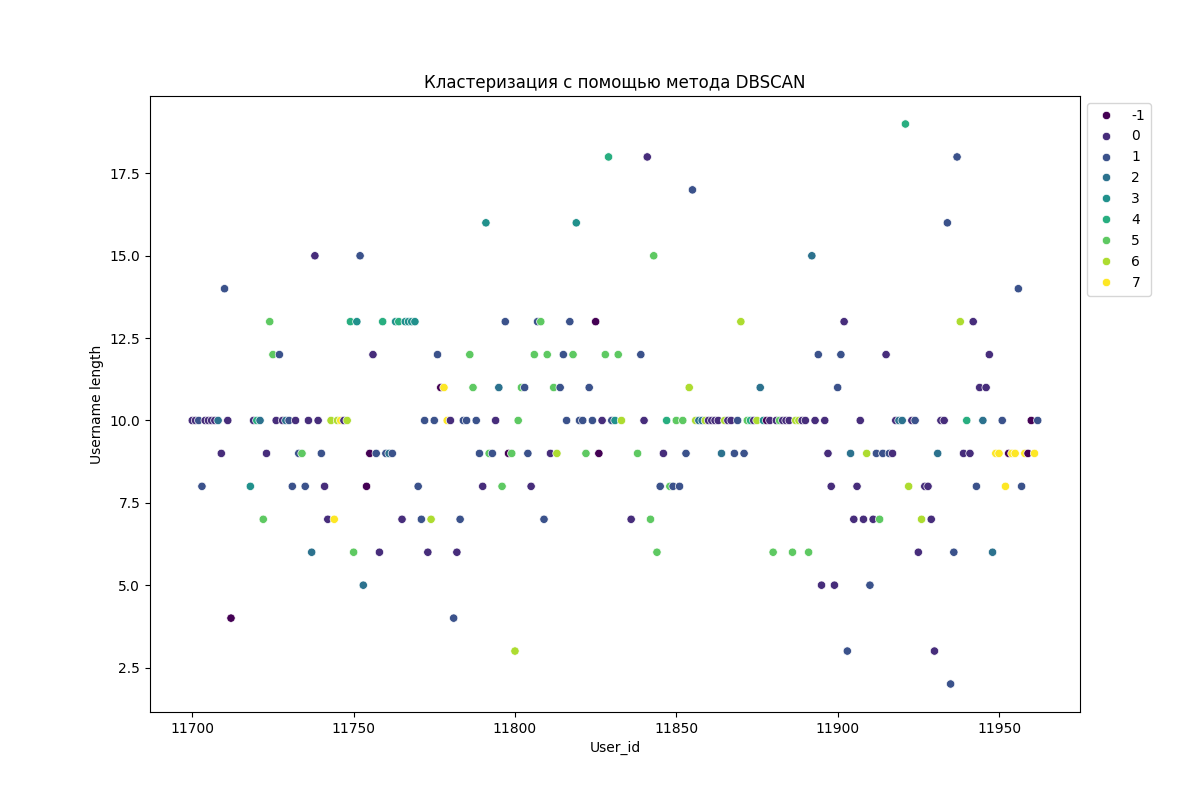
\includegraphics[scale=0.5]{Курсовая работа/pic/dbscan_clustering_ALL.png}
    \caption{Иерархическая кластеризация}
    \label{ris:dbscan}
\end{figure}

После этого были произведены расчеты метрик алгоритма, с использованием ячеек матрицы ошибок (табл. ~\ref{tabular:tableDBSCAN}). 

\begin{table}[!ht]
    \onehalfspacing \caption{Прогноз алгоритма}
    \medskip
        \begin{tabular}{|c|c|}
        \hline
            True Positive & 8\\  \hline 
            True Negative & 154\\  \hline 
            False Positive & 3\\  \hline 
            False Negative & 89\\  \hline 
        \end{tabular}
    \label{tabular:tableDBSCAN}
\end{table}

Для оценки качества работы алгоритма необходимо рассчитать ввести метрики accuracy (аккуратность), precision (точность) и recall (полнота).

$$
accuracy = \frac{TP+TN}{TP+TN+FP+FN} = 0,60
$$

$$
precision = \frac{TP}{TP+FP} =  0,3
$$

$$
recall = \frac{TP+TN}{TP+FN} = 0,03
$$

$$
F = 2\cdot \frac{precision \cdot recall}{precision+recall} = 0,05
$$


\vspace{1.5em}
\textbf{Сравнение трех алгоритмов}

Результаты рассчитанных метрик для всех реализованных алгоритмов представлены в таблице ~\ref{tabular:tableСomparison}.

\begin{table}[H]
    \onehalfspacing \caption{Метрики алгоритмов}
    \medskip
        \begin{tabular}{|c|c|c|c|c|}
        \hline
            \backslashbox{}{} & accuracy & precision & recall & F \\ \hline
            Isolation forest & 0,63 & 0,62 & 0,08 & 0,14 \\  \hline 
            Hierarchical clustering & 0,60 & 0,3 & 0,03 & 0,05 \\  \hline 
            DBSCAN & 0,64 & 0,78 & 0,07 & 0,13\\  \hline 
        \end{tabular}
    \label{tabular:tableСomparison}
\end{table}
